\part{Introduction and its Background}

\hspace\parindent
Over the years, technology has drastically changed our world and daily lives. It also became more personal and portable – as evident with the massive growth of individuals having personal computers. Nowadays, people are using computers to help them work or study, from communicating with someone, taking photos, searching information on the web, to even writing and creating a document electronically.

\hfill

One of the most useful functions of using an app on a computer is its capability of allowing an
individual to find words or phrases quickly in a full text, also known as the \textbf{full-text
search} feature. One popular function that uses the concept of full-text search is the keyboard shortcut “ctrl+f”. People often use this to find a specific phrase or characters in a long document or programs such as internet browsers, word processors, power point, etc.

\hfill

\textbf{Full-text search} is a method to search and locate a text pattern through the actual content of your computer documents (Full Text Search | FileCenter DMS, 2023; Full Text Search: How it Works, 2018). In this technique, the documents must have an actual text and not just scanned images. Therefore, if an individual can’t select and copy a text from the document, the text cannot be searched. This also means that a scanned document, scanned image, or any type of photos are not searchable even if it has text in it.

\hfill

In terms of implementing a full-text search feature into an application software, it is typical to
utilize a string-matching algorithm, such as the Boyer-Moore Algorithm, KMP Algorithm, Naïve
Algorithm, and Brute Force Algorithm. \textbf{String-matching algorithms} are algorithms that find
occurrences or matches of a pattern within a text or content of multiple files (GeeksforGeeks,
2022). With these string-matching algorithms, selecting one depends on the nature and requirements
of the software. As such, the study will utilize \textbf{Boyer-Moore Algorithm} as it is suitable for
pattern searching in huge bodies of text, and also the more efficient algorithm compared to other several
string-matching algorithms (Khumaidi et al., 2020; Layustira \& Istiono, 2021; Rasool et al., 2012; 
Supatmi \& Sumitra, 2019; Dawood \& Barakat, 2020; Lin \& Soe, 2020; Buslim et al., 2020; Borah et al., 2013).

\hfill

Since the Boyer-Moore Algorithm is a powerful and efficient string-matching algorithm, numerous existing studies and applications have implemented this algorithm for the full-text search feature of their software. However, based on the lack of resources and studies online, there is little to no applications that provide an in-image text searching feature utilizing Boyer-Moore as its string-matching algorithm. For instance, Waruwu (2017), Buslim et al. (2020), Khumaidi et al. (2020), and Layustira and Istiono (2021) did not use the Boyer-Moore algorithm to implement a text search feature for text patterns present in an image for their application software. In-image text search refers to the method of searching and extracting text within an image or multiple image files.

\hfill

To address this issue, the study will focus on developing an application software that has the capability of detecting and locating a text pattern within an image file using Boyer-Moore algorithm as the string-matching algorithm. The application will also be integrated with an optical character recognition (OCR) API to recognize and extract texts from images. Furthermore, a function that highlights the location of the text pattern in an image file or shows a message if the pattern is not detected will be implemented for the software.

\begin{figure}[hbt!]
   \center
   \noindent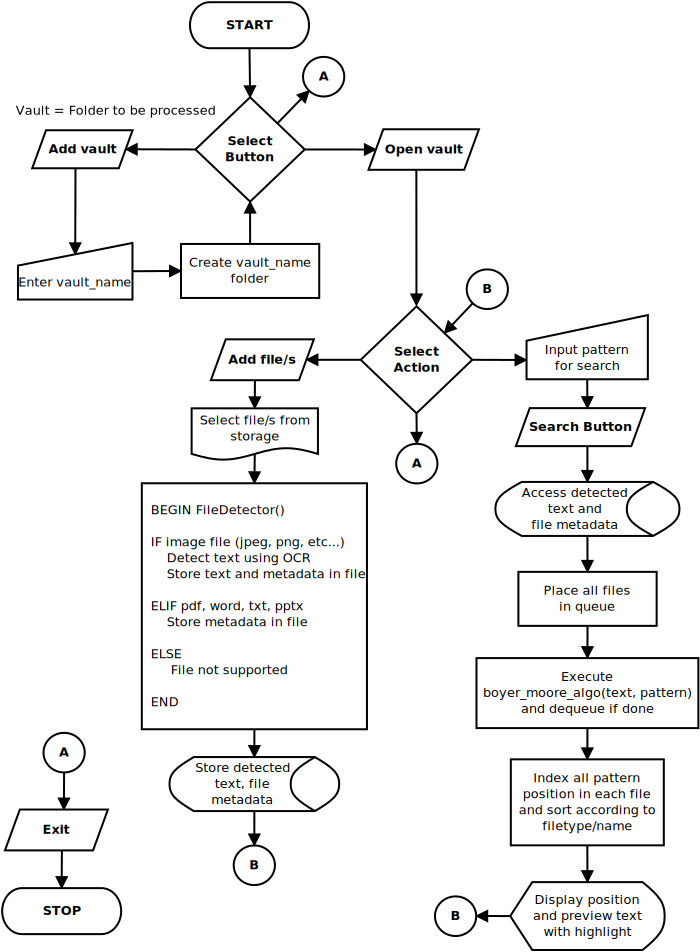
\includegraphics[width=0.9\textwidth]{figflowchart.png}
   \caption{Flowchart}
   \label{fig:flowchart}
\end{figure}
